\section*{Robot Arm Path Planning} 
If a robot manipulator is required to visit specific discrete points, waypoints, path planning is the problem of deciding how to move between these points. Planning the path is also important to ensure the movements are smooth, meaning that, since we "control" the speed of each joint, the desired positions and velocities should be continuous.%Path planning is very important, a smooth path will make a manipulator move better :) %is right
\subsection*{Interpolation}
One method of interpolating between points is to use cubic spline interpolation. A spline \cite{spline_wolfram} is a piecewise polynomial function and consequently a cubic spline is a function consisting of piecewise cubic polynomials. A cubic polynomial will ensure a smooth movement since its first derivative, the velocity, will be continuous. To ensure that each required point is visited the bounding values for each cubic function are set to zero \cite{cubic_spline_wolfram}.
\subsection*{Joint Space interpolation or Cartesian Motion}
The interpolation can take place in joint space or in cartesian space. Joint space interpolation means that the waypoints are expressed as joint values, angle of rotation if the joint is a revolute joint and distance if the joint is a prismatic joint.
The interpolation is then calculated between these joint values. Cartesian motion means that the waypoint are expressed as cartesian coordinates and that the interpolation takes place in cartesian space.
%Joint space - interpolate the joint values
%Cartesian motion - interpolate in 3D space -> convert to joint angles
\subsection*{Implementation} %Pre recorded path
The robotic manipulator, shown in figure \ref{fig:robotic_manipulator_general}, has a number of waypoints that it is required to visit. The desired waypoints are expressed in joint values, and a cubic spline interpolation is used to interpolate between these joint space waypoints. The path for picking up and placing the object can be seen in figure \ref{fig:pickup_path_interpolated} and \ref{fig:place_path_interpolated} respectively.

\begin{figure}[H]
    \centering
    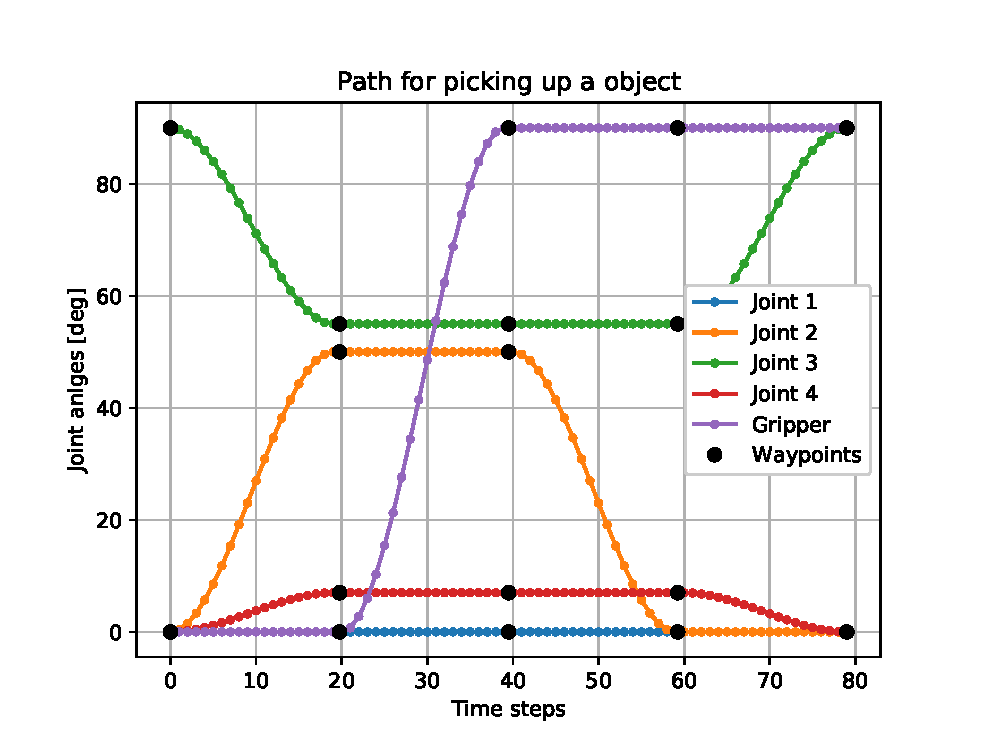
\includegraphics[width=0.5\textwidth]{chapters/img/pickup_path.eps}
    \caption{Path showing the joint values required for picking up the object.}
    \label{fig:pickup_path_interpolated}
\end{figure}


\begin{figure}[H]
    \centering
    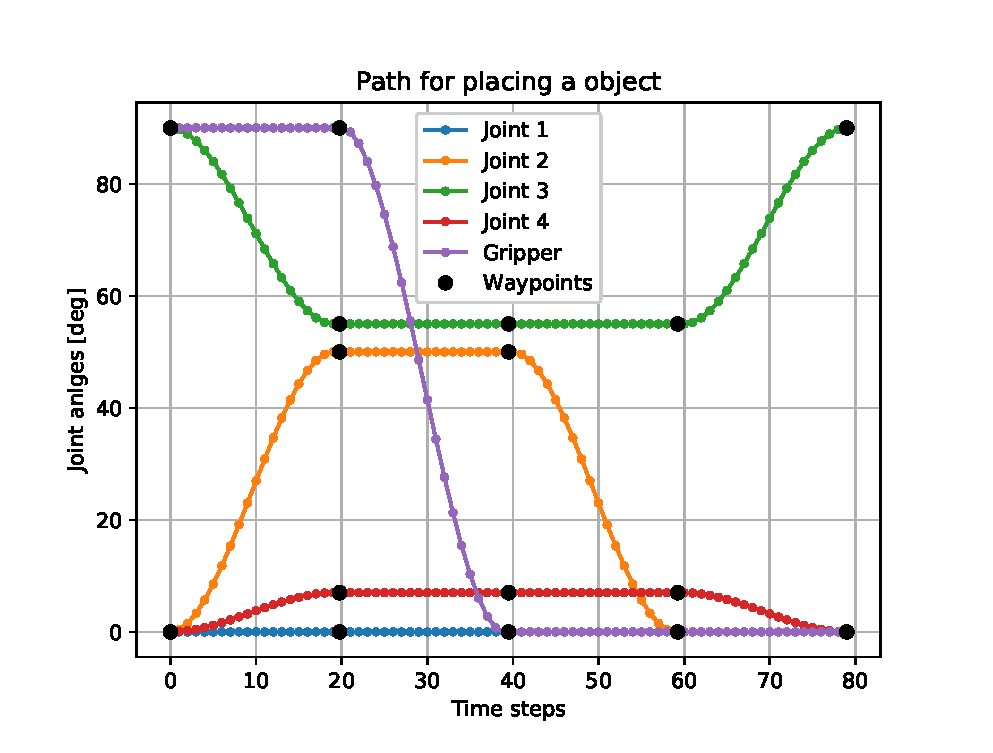
\includegraphics[width=0.5\textwidth]{chapters/img/place_path.eps}
    \caption{Path showing the joint values required for placing the object.}
    \label{fig:place_path_interpolated}
\end{figure}






\section*{Base}


